\chapter{Theoritical model of the human thigh expected impact on biped locomotion} % (fold)
\label{appendix:thigh_model}



If we look closely at the morphology of the human femur, it appears that it is inclined by an angle of 6\textsuperscript{o}. This makes the feet closer to the projection of the center of gravity (CoG) (see Fig.~\ref{fig:human_thigh}) and enhances stability  in  two main ways  during the walking gait:

\begin{itemize}
    \item As the feet are closer to the center of gravity, the lateral translation of the CoG necessary to transfer the mass of the robot from one foot to another is reduced (see Fig~\ref{fig:human_thigh}). In the case of Poppy's morphology, thanks to the $6$\textsuperscript{o} bended thigh, the lateral motion of the CoG is reduced by about 30\% ($ 5 cm$ instead of $7.1 cm$).
    \item During the stance phase, the CoG initial conditions are slightly modified. As we will explain with a simple theoretical model in the next section, the bended thigh can reduce the falling rate.
\end{itemize}


\begin{figure}[tb]
\centering
    \subfloat[][]{\label{fig:human_thigh}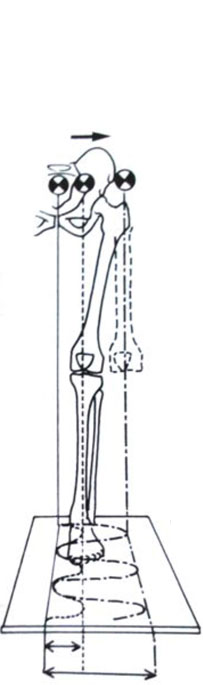
\includegraphics[height=8cm]{human_thigh.jpg}}
    \hfil
    \subfloat[][]{\label{fig:model_thigh}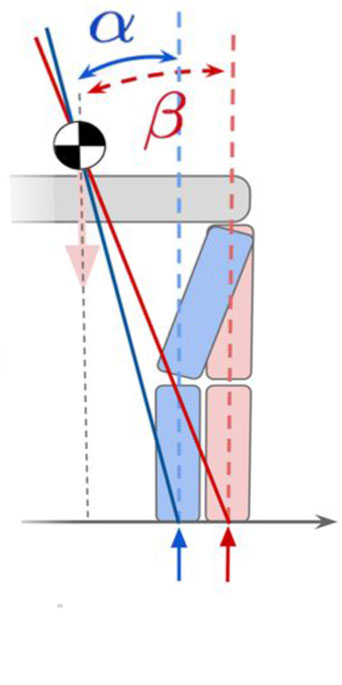
\includegraphics[height=8cm]{model_thigh.jpg}}
    \hfil
    \subfloat[][]{\label{fig:thigh_of_poppy}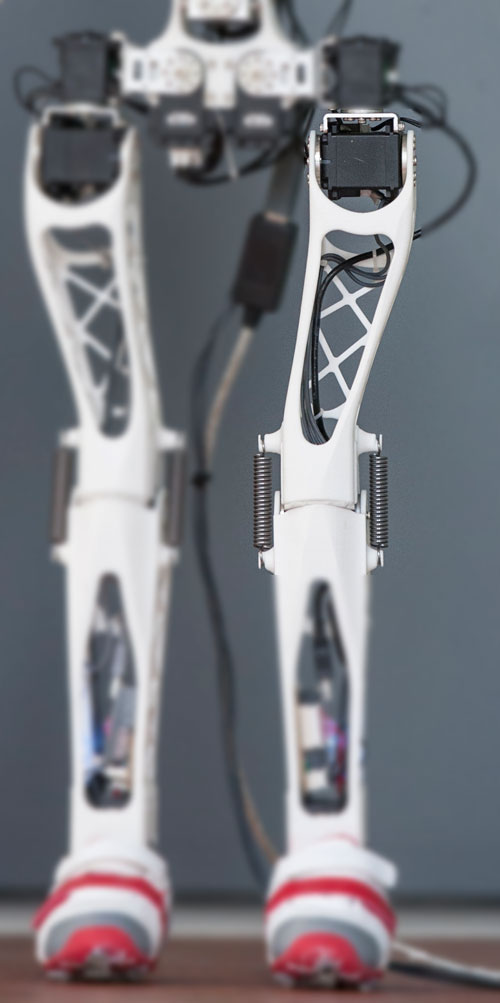
\includegraphics[height=6cm]{thigh_shape_large.jpg}}
    \caption{ a) Effect of bended human femur on human bipedal locomotion.
    b) Model used for the comparison of the two thighs morphology.
    c) Implementation of the bended thigh on the poppy platform}
    \label{fig:poppy_thigh}
\end{figure}

\section{Theoretical model} % (fold)
\label{sub:exp_theoritical_model}

We can model the situation where the robot is on one foot by an inverted pendulum with a mass point centered on the center of gravity (CoG) of the robot and the axis of rotation located at the foot position (see Fig.~\ref{fig:thigh_of_poppy}). With such a model, the dynamic of the whole structure depends on:

\begin{itemize}
    \item the length $l$ of the segment extending from the foot to the center of gravity,
    \item the angle $\theta$ of the segment relative to the vertical axis,
    \item the force of gravity $g$.
\end{itemize}

And the system follows this physical law:

\begin{equation}
    \ddot{\theta}(t) + w_0 \cdot sin(\theta(t)) = 0
\end{equation}
with:
\begin{equation}
    w_0 = \sqrt{\frac{g}{l}}
\end{equation}

\section{Intuitive expectation} % (fold)

To get an initial insight into this behavior, we can linearize the system for small disturbances such as:

\begin{equation}
    \theta(t) = \theta_0 \cdot cos(w_0\cdot t)
\end{equation}
and
\begin{equation}
    \dot{\theta}(t) = -\theta_0 \cdot w_0 \cdot sin(w_0\cdot t)
\end{equation}

One can see that the position and velocity of the pendulum varies linearly with the initial condition i.e $\theta$ angle. Therefore, reducing this initial angle $\theta_0$ involves a direct reduction of the falling speed $\dot{\theta}(t)$ of the robot.

In the case of Poppy's geometry, the thigh bending allows a 40\% reduction of the initial angle $\theta_0$ ($\alpha = 3.8$\textsuperscript{o} against $ \beta = 6.4$\textsuperscript{o} on Fig.~\ref{fig:model_thigh}).

\section{Simulation} % (fold)

In the case of a fall, it is not possible to assume small perturbations, that is the reason why we have simulated the model in Matlab with a non-linear system and obtain the behavior represented in Fig.~\ref{fig:dynamic_thigh_model}.

\begin{figure}[thpb]
    \centering
    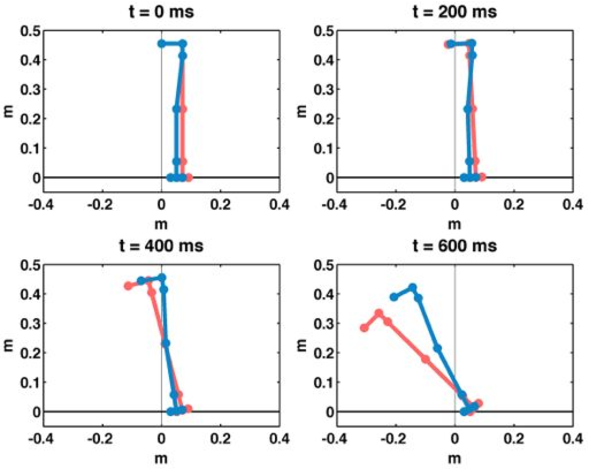
\includegraphics[width=0.8\linewidth]{dynamic_thigh_model.pdf}
    \caption{Comparison of the falling dynamic over time when Poppy is standing on one foot, depending on its thigh morphology: with a bended thigh of 6\textsuperscript{o} (blue) and with a straight thigh (red).}
    \label{fig:dynamic_thigh_model}
\end{figure}

If we define the center of gravity altitude as:
\begin{equation}
    z_{CoG} = l \cdot cos(\theta(t))
\end{equation}
We can express its falling speed over time as:
\begin{equation}
    \dot{z}_{CoG} = - \dot{\theta}(t) \cdot l \cdot sin(\theta(t))
\end{equation}

In this condition, if we consider the first 700 ms of the system behavior simulation and compare the two systems, the mean of the CoG falling speed is reduced by around 56\% in the bended thigh case.


